\section{开始使用}\label{sec:intro}

\par 这一章的主要目的是为了介绍什么是\LaTeX,\verb|sicnu.cls|文档类的基本使用方法以及整个项目的布局。顺便生成一些表格和图片便于测试整个文档以及用户快速对模板的修改和使用。

\subsection{什么是\LaTeX }\label{sec:intro:p1}
\par TEX是高德纳(Donald E. Knuth)为排版文字和数学公式而开发的软件\cite{texbook}。\LaTeX 是一种使用TEX程序作为排版引擎的格式,可以粗略地将它理解成是对TEX的一层封装。我们当前使用的版本是\LaTeXe,事实上{\LaTeX}3已经发布很多年了,但是\LaTeXe 仍然是目前使用最广泛的版本。点击\href{https://www.latex-project.org/latex3/}{传送门}查看关于{\LaTeX}3的更多信息。

\par 下面介绍常见的\LaTeX 引擎, \LaTeX 发行版以及 \LaTeX 编辑器的区别与联系。请看图\ref{fig:texbase}:
\begin{figure}[H]
    \centering
    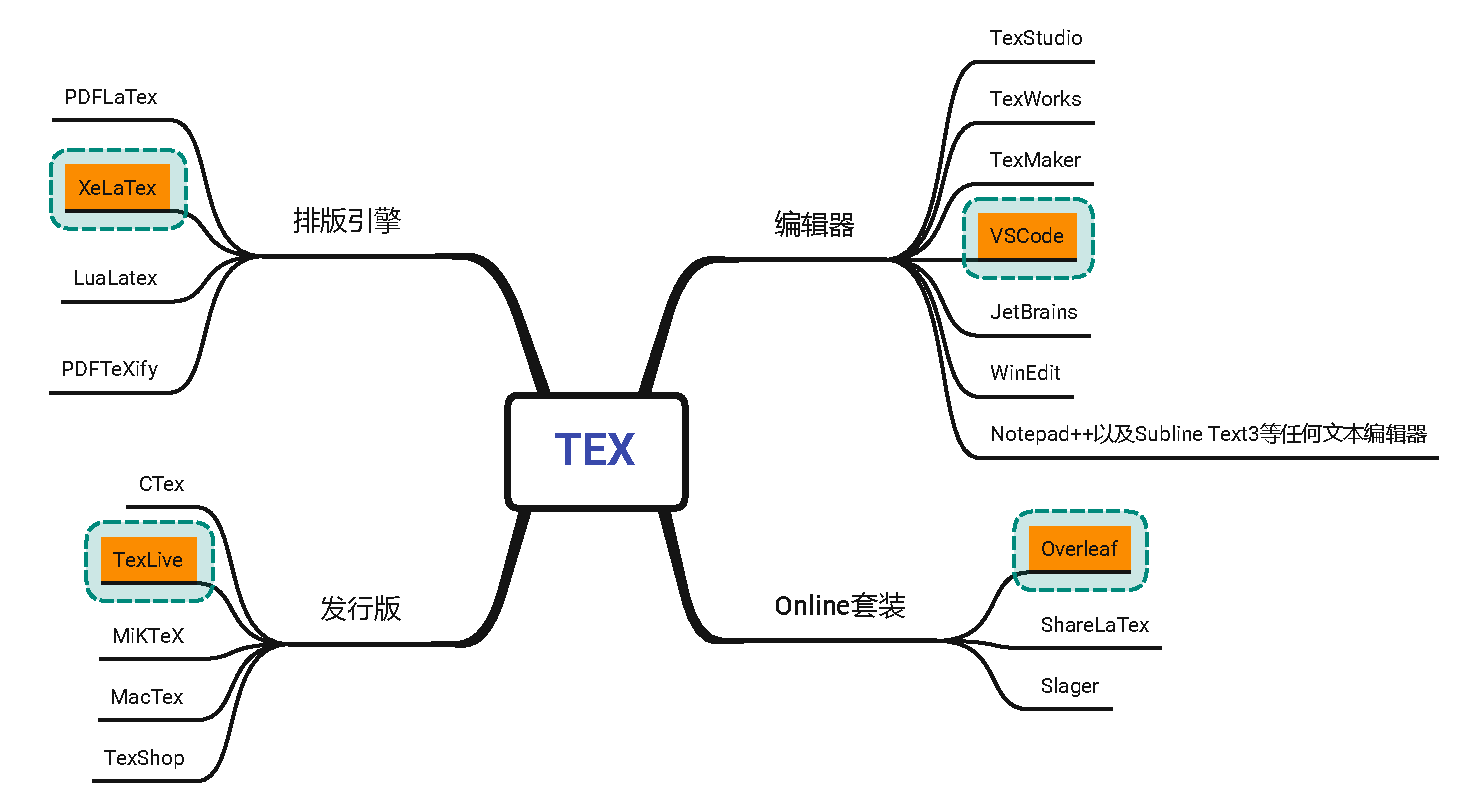
\includegraphics[scale=0.5]{./img/TEX.pdf}
    \caption{TeX的基础知识}
    \label{fig:texbase}
\end{figure}

\par \textcolor{red}{这个项目使用的\LaTeX 发行版为TeXLive2021,编译引擎为XeLaTex,开发环境为VSCode。}需要注意的是,尽管TeXLive支持macOS和Linux,但TeX并不是一个跨平台语言,\textcolor{red}{所以Mac和Linux用户将无法轻松的使用这个模板。}如果你要使用这个模板,下面的条件需要尽可能的满足:

\begin{tcolorbox}[colback=gray!10,
    colframe=black,
    width=16cm,
    arc=1mm, auto outer arc,
    boxrule=0.5pt,]
    \begin{itemize}
        \item 操作系统为Windows7以上。
        \item $\mathrm{TexLive~~Version >= 2021}$,更高或更低的版本也应该能完成编译,这只是成功的充分条件,但是禁用CTex。
        \item 编辑器推荐等级:$\mathrm{VSCode > TexStudio > TexWorks > TexMaker}$,其中TeXLive自带TexWorks编辑器。禁用WinEdit。
        \item 编译方式为XeLaTex。
        \item 如果你不想安装TeXLive,请使用\textcolor{red}{Overleaf或ShareLaTex},通过它们你可以直接从\href{github}{github}上导入这个项目在线编译。
    \end{itemize}
\end{tcolorbox}
如果你点电脑上没有安装TeXLive,请查看\href{https://www.bilibili.com/video/BV1tg4y1B7f3/?spm_id_from=333.337.search-card.all.click&vd_source=758c464d5854d0b3d36de4033fcbdc7a}{\LaTeX 工作室}制作的安装教程:\url{https://www.bilibili.com/video/BV1tg4y1B7f3/?spm_id_from=333.337.search-card.all.click&vd_source=758c464d5854d0b3d36de4033fcbdc7a}。这个教程前半部分介绍TeXLive的安装,后半部分介绍了命令行的用法,只需要完成前半部分教程即可。

\subsection{sicnu.cls的基本用法}

\par \verb|sicnu.cls|文件目前包括新定义了$29$个可供直接调用的外部指令,新定义了$5$个的环境,重定义了$7$个环境。内部命令和宏不在此处列出,如果有这些定义解决不了的问题请查看源码。图\ref{fig:basevar}是主程序入口,它的结构不会因为你的论文内容而改变。
\begin{figure}[H]
    \centering
    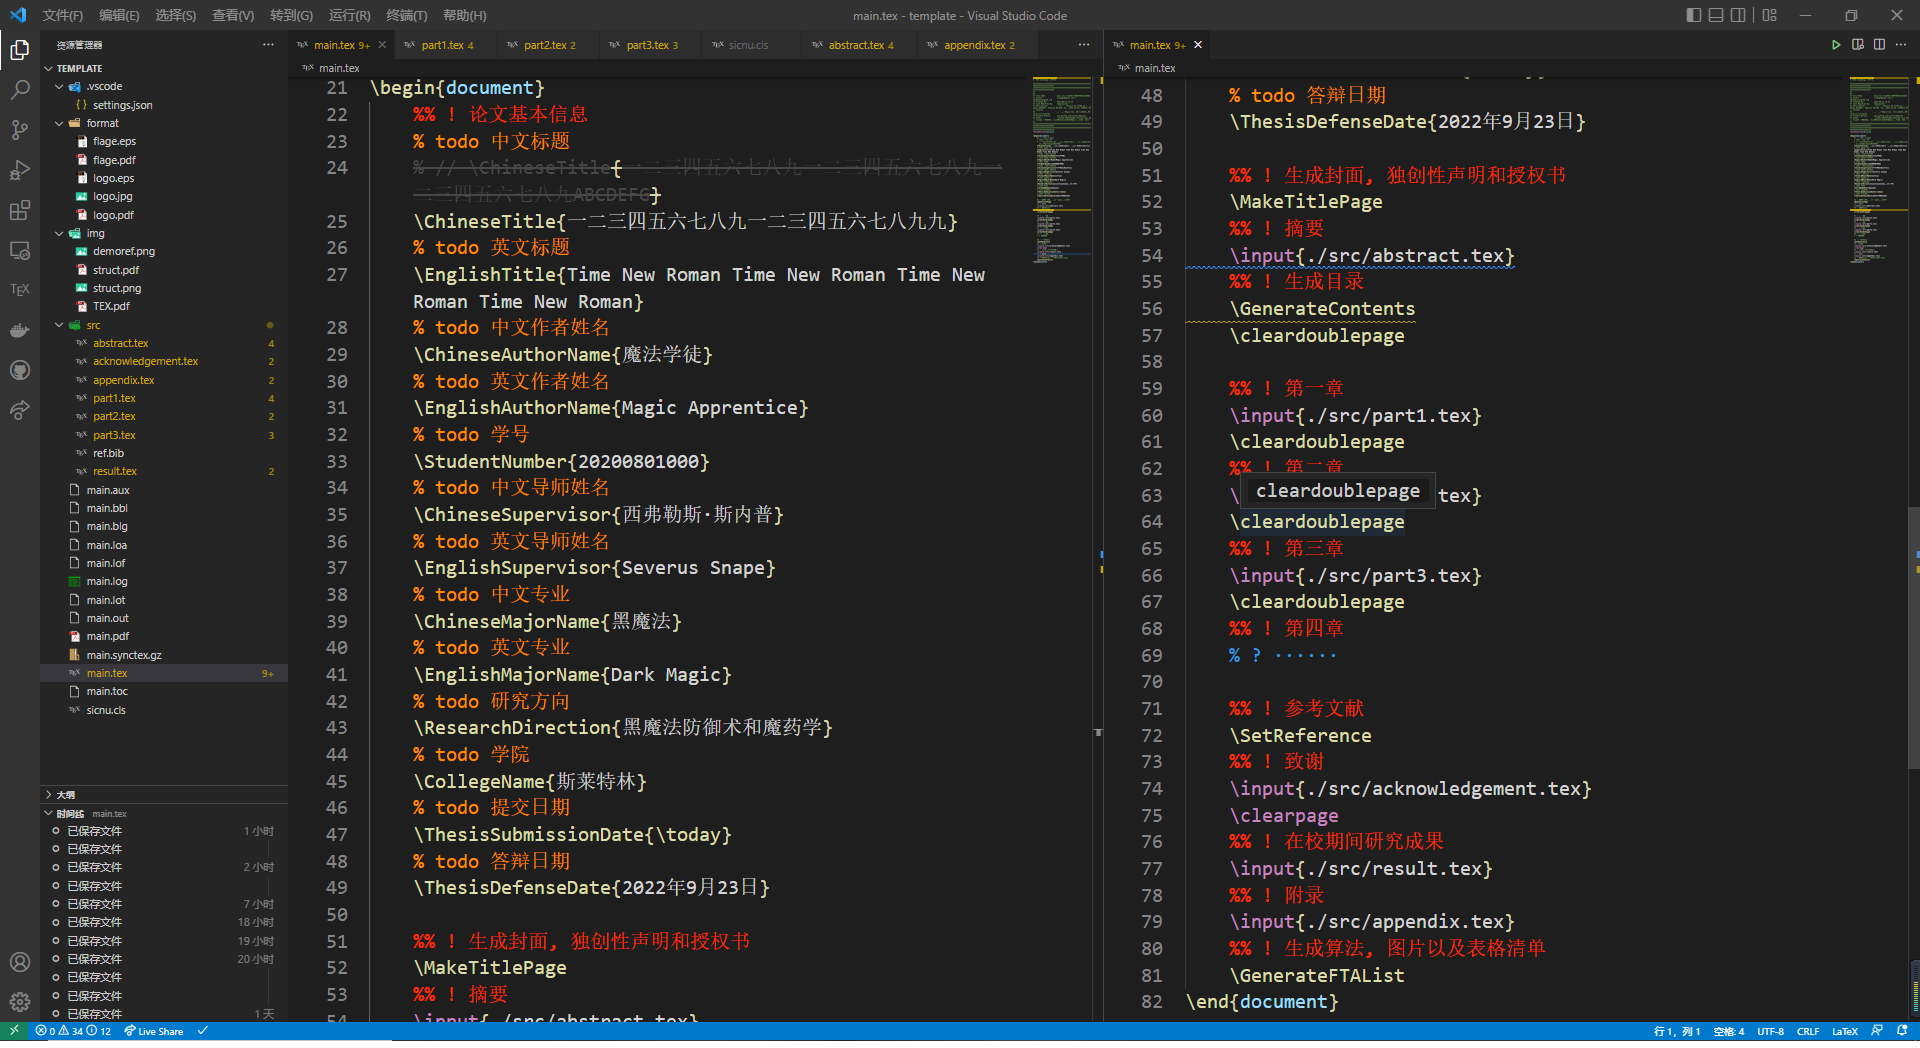
\includegraphics[scale=0.3]{img/struct.png}
    \caption{文档的基本元素设置}
    \label{fig:basevar}
\end{figure}
以上这些命令都是最基本的命令,你无需记住它,而它们也只会使用一次。看懂了这张图,那么这个模板你已会$80\%$了。诸如分类号和学校代码等也提供了指令修改它,但是默认值就是SICNU,故无特殊需要可以不用在意它。第二章会列出所有可供调用的指令和环境,以供后期调试和使用。

\subsection{项目布局}
\par 也许你已经发现了,图\ref{fig:basevar}中并没有任何正文的内容。它们都是通过如第$58$行的\verb|\input{path}|导入相应的文件。文章的每一章都将使用一个独立的文件保存,而不是一股脑的把所有内容塞到一个文件中,这将方便我们检查错误和提高专注力。结合图\ref{fig:basevar}和图\ref{fig:projstru}以及你的论文,你就知道你需要修改模板的哪个地方了。

\begin{figure}[H]
    \centering
    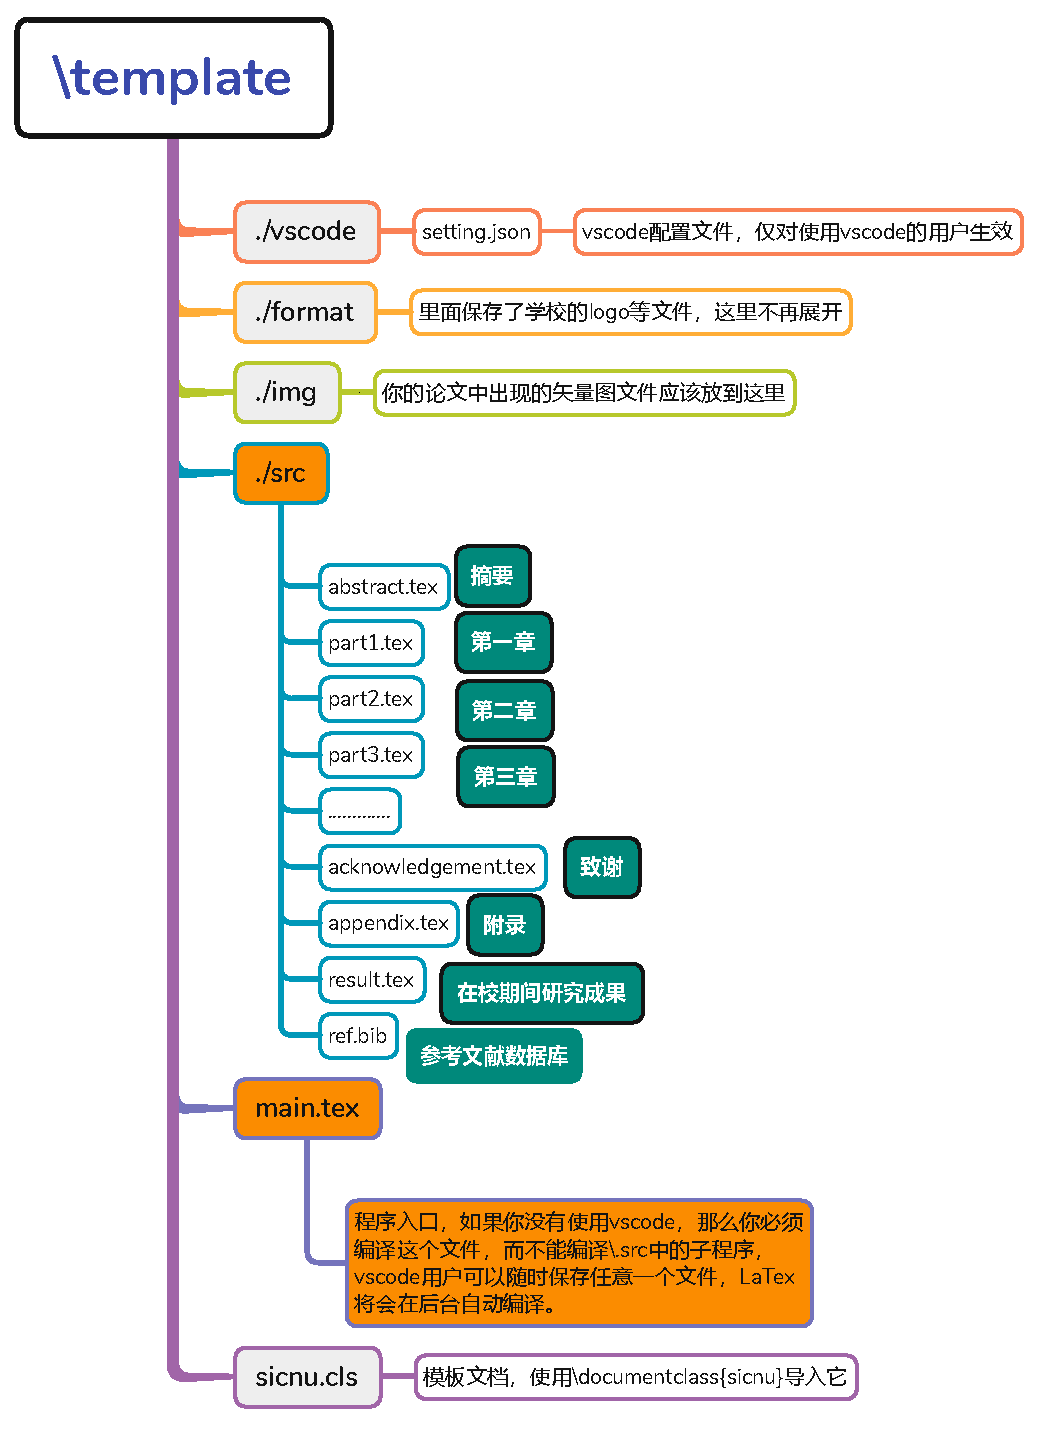
\includegraphics[scale=0.8]{img/struct.pdf}
    \caption{项目布局}
    \label{fig:projstru}
\end{figure}

\subsection{轻松引用参考文献}
看到这里,你已经学会了这个模板$90\%$的内容了。接下来,学习如何使用数据库来管理你的参考文献。\textcolor{red}{使用数据库管理和引用参考文献的方式可以避免手动输入文献和文献引用排序的问题,这是以前的CTex模板最让人难以忍受的地方。}将你的参考文献放到\verb|ref.bib|文件中,形如:
\begin{tcolorbox}[colback=gray!10,
    colframe=black,
    width=16cm,
    arc=1mm, auto outer arc,
    boxrule=0.5pt,]
    \begin{verbatim}
        % ./src/ref.bib
        @article{tpe,  % 引用的别名
            title={Algorithms for hyper-parameter optimization},
            author={Bergstra, James and Bardenet,
                R{\'e}mi and Bengio, Yoshua and K{\'e}gl, Bal{\'a}zs},
            journal={Advances in neural information processing systems},
            volume={24},
            year={2011}
        }
        @article{lecun, % 引用的别名
            title={Deep learning},
            author={LeCun, Yann and Bengio, Yoshua and Hinton, Geoffrey},
            journal={nature},
            volume={521},
            number={7553},
            pages={436--444},
            year={2015},
            publisher={Nature Publishing Group}
        }
    \end{verbatim}
\end{tcolorbox}
这些信息非常容易获取,知网,百度学术,Google Scholar都有复制粘贴的选项,如图\ref{fig:citebib}所示。
\begin{figure}[H]
    \centering
    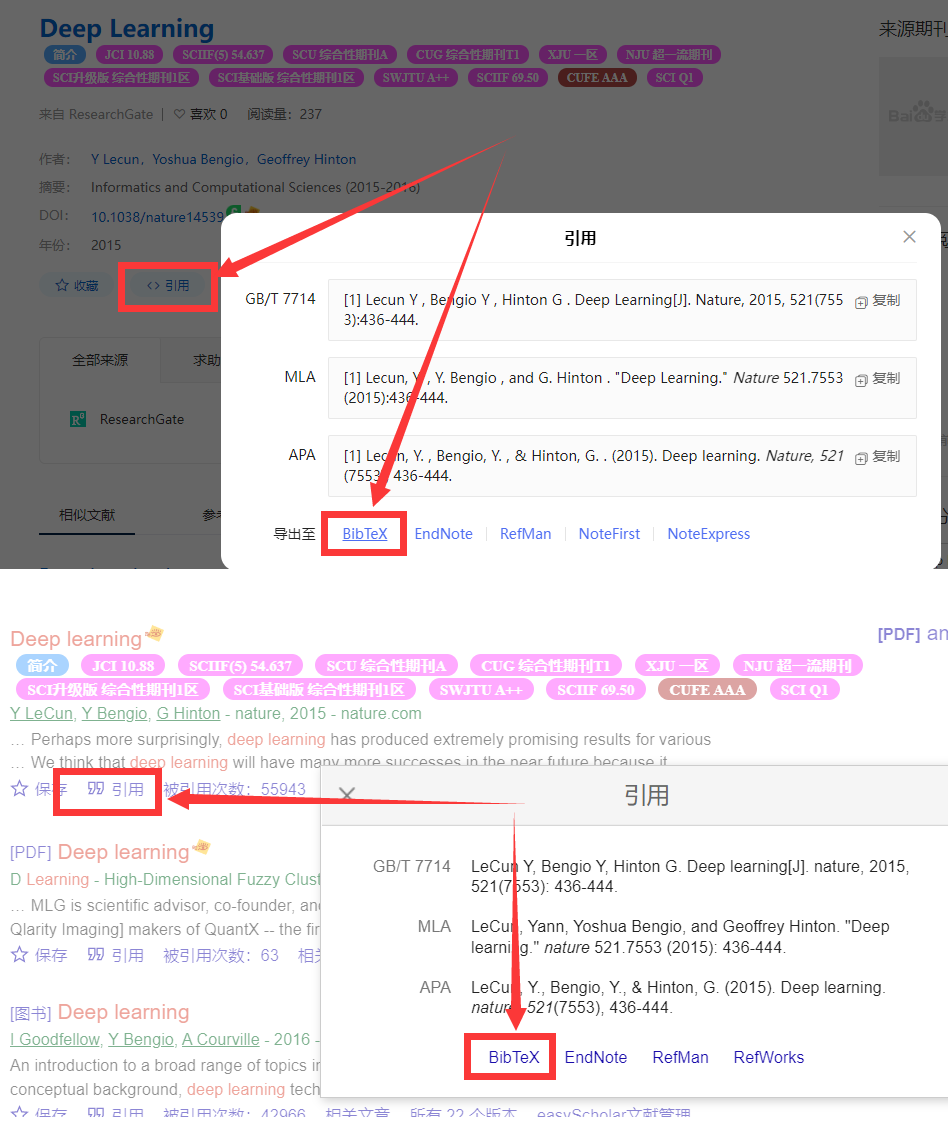
\includegraphics[scale=0.3]{img/demoref.png}
    \caption{如何复制参考文献的引用格式}
    \label{fig:citebib}
\end{figure}

将bib格式的文献复制粘贴到\verb|ref.bib|文件中后,接下来使用\verb|\cite{tpe, lecun}| \cite{tpe, lecun}引用这两个文献。使用这种方式引用文献有以下好处,这是之前CTex模板没有解决的问题:
\begin{tcolorbox}[colback=gray!10,
    colframe=black,
    width=16cm,
    arc=1mm, auto outer arc,
    boxrule=0.5pt,]
    \begin{itemize}
        \item 文献会根据你在正文中引用的顺序自动在末尾产生参考文献页。(以前的模板需要手动排序,比如你在第$7$个文献后又引用了一个新的文献,那么后面的文献你都要手动把序号$+1$。现在,你只管引用,文献排序将自动完成。)
        \item 文献引用规范为(GB/T 7714--2005),以前的模板有的没有遵循这个规则。
        \item 使用数据库管理文献避免了你去手动排版文献格式,复制粘贴更不容易出错。
    \end{itemize}
\end{tcolorbox}

